% Copyright Aidan Randle-Conde 2007-2014
% http://www.aidansean.com/phd_notes
% Anyone is free to download, redistribute, edit and use these notes and the source tex files with the following restrictions:
% This 
%  This message is included in the tex source files.
%  Aidan Randle-Conde is credited as the author.
%  Images are correctly credited to their respective authors, as outlined in the references.
%  No part of these notes may be used for commercial purposes.

\chapter{Spontaneous symmetry breaking}

It is desirable to add mass to the theory of the Standard Model, as the $W$ and $Z$ are not massless.  However, simple mass terms cannot be added by hand to the Lagrangian (as is done with the Klein-Gordon equation) as the theory is not renormalisable.  So the particle mass is generated by ``spontaneous symmetry breaking''.

Before considering Weinberg's model of the Higgs mechanism as applied to the electroweak sector, consider some ``toy'' models:

\begin{enumerate}
  \item Spontaneous symmetry breaking for a scalar field $\phi$ for which $\phi \to -\phi$ is a symmetry
  \item Spontaneous symmetry breaking in a complex scalar field which has a global gauge symmetry (Goldstone boson)
  \item Spontaneous symmetry breaking in a complex scalar field which has a local gauge symmetry.  The electromagnetic-like field introduced to allow invariance with respect to local gauge transformation cures the Goldstone boson problem and the $A^{\mu}$ field acquires mass (the Higgs model, 1984).
\end{enumerate}

Consider the Lagrangian for a free scalar field:

\[
  L = \frac{1}{2}\left(\partial_{\mu}\phi\right)^2 - \left(\frac{1}{2}\mu^2\phi^2 + \frac{\lambda}{4}\phi^4\right)
\]

where $\lambda>0$.  This Lagrangian is symmetric under the transformation $\phi \to -\phi$.  If $\mu^2>0$ there is a minimum at $\phi = 0$ (ground state vacuum) and the $\phi^4$ is a self interacting term allowing a four-particle vertex.

If $\mu^2<0$ the potential has two minima:

\begin{eqnarray*}
  \frac{\partial V}{\partial\phi} & = & \mu^2\phi + \lambda \phi^3 \\
  & = & 0 \\
  \Rightarrow \phi^2_{min} & = & -\frac{\mu^2}{\lambda} \\
  \textrm{so } \phi_{\min} & = & \pm\sqrt{-\frac{\mu^2}{\lambda}} \\
  & = & \pm \nu
\end{eqnarray*}

where $\nu$ is the vacuum expectation of the field.  Consider the potential at the minimum $\phi$:

\begin{eqnarray*}
  V & = & \frac{\mu^2}{2}\phi^2 + \frac{\lambda}{4}\phi^4 \\
    & = & \lambda\left( \frac{\mu^2}{2\lambda}\phi^2 + \frac{\phi^4}{4}\right) \\
    & = & -\frac{\lambda}{4}\nu^4
\end{eqnarray*}

\begin{figure}[!htb]
  \begin{center}
    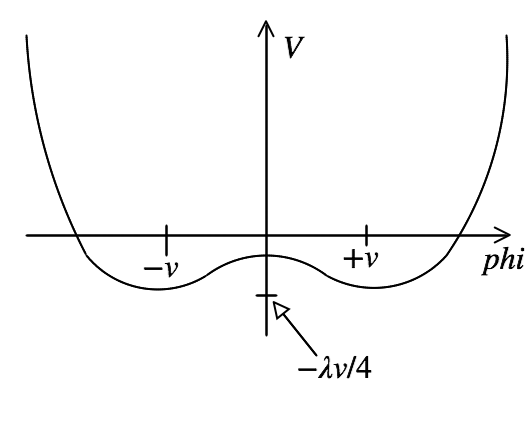
\includegraphics[width=0.75\textwidth]{images/web_feynman/image_83.png}
    \caption[The BEH potential]{The Brout-Englert-Higgs potential}
    \label{fig:ch16_potential}
  \end{center}
\end{figure}

Perturbative expansion should be around the classical minimum, $\phi = \nu$ or $\phi = -\nu$:

\[
  \phi(x) = \nu + \eta(x)
\]

where $\eta(x)$ represents the quantum fluctuations about this minimum.  Substituting this into the Lagrangian:

\begin{eqnarray*}
  L' & = & \frac{1}{2}\left(\partial_{\mu}\eta\right)^2 - \left(\frac{1}{2}\mu^2\left(\nu + \eta(x)\right)^2 + \frac{1}{4}\lambda\left(\nu + \eta(x)\right)^4\right) \\
  & = & \frac{1}{2}\left(\partial_{\mu}\eta\right)^2 - \left(\frac{1}{2}\mu^2\left(\nu^2 + 2\nu\eta + \eta^2\right) + \frac{1}{4}\lambda\left(\nu^4 + 4\nu^3\eta + 6\nu^2\eta^2 + 4\nu\eta^3 + \eta^4\right)\right) \\
  \textrm{But } \mu^2 & = & -\nu^2\lambda \\
  L' & = & \frac{1}{2}\left(\partial_{\mu}\eta\right)^2 - \left(-\frac{1}{2}\lambda\nu^4 - \lambda\eta\nu^3 - \frac{1}{2}\lambda\nu^2\eta^2 + \frac{1}{4}\lambda\nu^4 + \lambda\eta\nu^3 + \frac{3}{2}\lambda\eta^2\nu^2 + \lambda\nu\eta^3 + \frac{1}{4}\lambda\eta^4\right) \\
  & = & \frac{1}{2}\left(\partial_{\mu}\eta\right)^2 - \left(\lambda\nu^2\eta^2 + \lambda\nu\eta^3 + \frac{1}{4}\lambda\eta^4 + constant\right)
\end{eqnarray*}

The field $\eta$ has a msss term of the correct sign.  Identifying with the Klein-Gordon mass term, $-\frac{1}{2}m^2\phi^2$, this means:

\begin{eqnarray*}
  -\lambda\nu^2 & = & -\frac{1}{2}m_{\eta}^2 \\
  \Rightarrow m_{\eta} & = & \sqrt{2\lambda\nu^2} \\
  & = & \sqrt{-2\mu^2}
\end{eqnarray*}

The method of arbitrarily choosing one of the states as the ground states ie $\phi = +\nu $ and not $\phi = -\nu$, is called spontaneous symmetry breaking.

For a complex field:

\[
  \left(\phi_1^2 + \phi_2^2\right) = -\frac{\mu^2}{\lambda} = \nu^2
\]

This is invariant under $\phi' = \e^{i\alpha}\phi$ ie invariant with respect to a global gauge transformation.  Again, for $\lambda>0$, $\mu<0$.

\[
  L = \frac{1}{2}\left(\partial_{\mu}\phi_1\right)^2 + \frac{1}{2}\left(\partial_{\mu}\phi_2\right)^2 -\frac{1}{2}\mu^2\left(\phi_1^2 + \phi_2^2\right) - \frac{\lambda}{4}\left(\phi_1^2 + \phi_2^2\right)^2
\]

There is now a circle of minima and the symmetry is broken by choosing $\phi_1 = \nu$ and $\phi_2 = 0$.  Then expand about the vacuum using:

\[
  \phi(x) = \frac{1}{\sqrt{2}}\left(\nu + \eta(x) + i\rho(x)\right) \\
\]

Putting the field, $\phi$, into $L$:

\begin{eqnarray*}
  L & = & \left(\partial_{\mu}\phi\right)^{\star}\left(\partial_{\mu}\phi\right) - \mu^2\phi^{\star}\phi - \lambda\left(\phi^{\star}\phi\right)^2 \\
  \Rightarrow L' & = & \frac{1}{2}\left(\partial_{\mu}\eta\right)^2 + \frac{1}{2}\left(\partial_{\mu}\rho\right)^2 + \mu^2\eta^2 + O(\eta^3) + O(\rho^3) + constant
\end{eqnarray*}

The third term again looks like a mass term of the form $\left(-\frac{1}{2}m_{\eta}^2\eta^2\right)^2$ with $m_{\eta} = \sqrt{-2\mu^2}$

So there is a kinetic energy term for the $\rho$ field but no mass term.  So in an attempt to break the symmetry a new term must be introduced.

\section{The Higgs model}

There is a complex field:

\[
  \frac{1}{\sqrt{2}}\left(\phi_1 + \phi_2\right)
\]

and the Lagrangian is required to be invariant with respect to a local gauge transformation.  To achieve invariance, the electromagnetic field, $A^{\mu}$ had been previously introduced and $\partial_{\mu} \to \partial_{\mu} - i\e A^{\mu}$.

The Lagrangian is:

\[
  L = \left(\partial^{\mu} + i\e A^{\mu}\right)\phi^{\star}\left(\partial_{\mu} - i\e A^{\mu}\right)\phi - \mu^2 \phi^{\star}\phi - \lambda\left(\phi^{\star}\phi\right)^2 - \frac{1}{4}F_{\mu\nu}F^{\mu\nu}
\]

For $\mu^2>0$ this is simply the QED Lagrangian for a charged scalar particle of mass $\mu$ (with a self-interaction term).  However, consider $\mu^2<0$ to spontaneously break symmetry.

It is possible to substitute $\phi = \frac{1}{\sqrt{2}}\left(\nu + \eta(x) + 1\rho(x)\right)$ into the Lagrangian, but a more subtle approach is:

\begin{eqnarray*}
  \phi & \simeq & \frac{1}{\sqrt{2}}\left(\nu + \eta(x)\right) \e^{i\rho(x)/\nu} \\
  & & \left( \rho(x)\eta(x) \textrm{ is small}\right)
\end{eqnarray*}

Note that $\e^{i\rho(x)/\nu}$ represents a local gauge transformation.  This implies that:

\begin{eqnarray*}
  \phi & \to \phi' & = \frac{1}{\sqrt{2}}\left(\nu + \eta(x)\right) \e^{i\rho(x)/\nu} \\
  A_{\mu} &\to A_{\mu} & = A_{\mu} + \frac{1}{\e}\partial_{\mu} \frac{\rho(x)}{\nu}
\end{eqnarray*}

The symmetry is broken by choosing $\rho(x) = 0$.  When the symmetry is broken:

\[
  \phi = \frac{1}{\sqrt{2}}\left(\nu + h(x)\right)
\]

where $h(x)$ is the Higgs term.  The Lagrangian becomes:

\begin{eqnarray*}
  L' & = & \left(\partial^{\mu} + i\e A^{\mu}\right)\left(\frac{\nu + h(x)}{\sqrt{2}}\right)\left(\partial_{\mu} - i\e A_{\mu}\right)\left(\frac{\nu + h(x)}{\sqrt{2}}\right)\\
  & - & \mu^2\left(\frac{\nu + h(x)}{\sqrt{2}}\right)^2 - \lambda\left(\frac{\nu + h(x)}{\sqrt{2}}\right)^2 - \frac{1}{4}F_{\mu\nu}F^{\mu\nu}
\end{eqnarray*}

Multiplying the terms out:

\[
  L' = \frac{1}{2}\left(\partial^{\mu}h\right)^2 - \lambda\nu^2h^2 + \frac{1}{2}\e^2\nu^2A_{\mu}A^{\mu} - \frac{1}{4}F_{\mu\nu}F^{\mu\nu} + \textrm{ other terms}
\]

The Lagrangian describes two interacting massive particles: a vector gauge boson $A_{\mu}$ and a massive scalar $h$, which is the Higgs particle.

\subsection[Weinberg formulation of the Higgs mechanism for \texorpdfstring{$SU(2) \otimes U(1)$}{SU2TimesU1}]{The Weinberg formulation of the Higgs mechanism for \texorpdfstring{$SU(2) \otimes U(1)$}{SU2TimesU1}}

Weinberg chose a weak isospin doublet of complex scalar fields with hypercharge $Y = 1$:

\[
  \begin{array}{cccc}
    &
    I_3 & Q & Y \\
    \phi = 
    \left(
    \begin{array}{c}
      \phi^+(x) \\
      \phi^0(x)
    \end{array}
    \right)
    &
    1/2  & 1 & 1 \\
    & -1/2 & 0 & 1
  \end{array}
\]

\begin{eqnarray*}
  \phi^{+} & = & \frac{\phi_1 + i\phi_2}{\sqrt{2}} \\
  \phi^{0} & = & \frac{\phi_3 + i\phi_4}{\sqrt{2}}
\end{eqnarray*}

The above scalar field was required to be invariant with respect to local gauge transformations in the weak isospin hypercharge space of the electroweak interaction.  Under such transformations the doublet transforms as:

\[
  \left(
  \begin{array}{c}
    \phi^+ \\
    \phi^0
  \end{array}
  \right)
  \to
  \left(
  \begin{array}{c}
    \phi^+ \\
    \phi^0
  \end{array}
  \right)'
  =
  \e^{ig_W\frac{\tau}{2}\alpha(\ul{r}) + i\frac{g'}{2}Y\beta(\ul{r})}
  \left(
  \begin{array}{c}
    \phi^+ \\
    \phi^0
  \end{array}
  \right)
\]

For the Lagrangian to be invariant $\partial_{\mu}$ has to be replaced by $D_{\mu}$.

The original Lagrangian is:

\[
  L = \left(\partial_{\mu}\phi\right)^{\dagger}\left(\partial^{\mu}\phi\right) - \mu^2 \phi^{\dagger}\phi - \lambda\left(\phi^{\dagger}\phi\right)^2
\]

So now:

\[
  L = \left| \left(\partial_{\mu} - \frac{g_W\tau}{2}W_{\mu} - \frac{g'}{2}YB_{\mu}\right)\phi\right|^2 - \mu^2\phi^{\dagger}\phi - \lambda\left(\phi^{\dagger}\phi\right)^2
\]

Weinberg broke the symmetry by setting:

\[
  \frac{1}{\sqrt{2}}
  \left(
  \begin{array}{c}
    \phi^+ \\
    \phi^0
  \end{array}
  \right)
  =
  \frac{1}{\sqrt{2}}
  \left(
  \begin{array}{c}
    0 \\
    \nu + h(x)
  \end{array}
  \right)
\]

From past experience of the various models discussed the boson masses come from the gauge terms in the $D_{\mu}$ operation.

The term is:

\begin{eqnarray*}
  & &
  \left| g_W \frac{1}{2}\left[
  \left(
  \begin{array}{cc}
    0 & 1 \\
    1 & 0
  \end{array}
  \right)
  W_{\mu}^1 +
  \left(
  \begin{array}{cc}
    0  & i \\
    -i & 0
  \end{array}
  \right)
  W_{\mu}^2 +
  \left(
  \begin{array}{cc}
    1 & 0 \\
    0 & -1
  \end{array}
  \right)
  W_{\mu}^3
  + \frac{g'}{2}
  \left(
  \begin{array}{cc}
    1 & 0 \\
    0 & 1
  \end{array}
  \right)
  B_{\mu}
  \right]
  \frac{1}{\sqrt{2}}
  \left(
  \begin{array}{c}
    0 \\
    \nu
  \end{array}
  \right)
  \right|^2
  \\
  & = & \frac{1}{8}\left|
  \left(
  \begin{array}{cc}
    g_W W_{\mu}^3 + g'B_{\mu} & g_W\left(W{\mu}^1 + iW_{\mu}^2\right) \\
    g_W \left(W_{\mu}^1 - iW_{\mu}^2\right) & -g_W W_{\mu}^3 + g'B_{\mu}
  \end{array}
  \right)
  \left(
  \begin{array}{c}
    0 \\
    \nu
  \end{array}
  \right)
  \right|^2
  \\
  & = & \frac{1}{8}\left(\nu g_W\left(W_{\mu}^1 - iW_{\mu}^2\right) , -\nu g_W W_{\mu}^3 + \nu g'B_{\mu}\right)
  \left(
  \begin{array}{c}
    \nu g_W\left(W_{\mu}^1 + iW_{\mu}^2\right) \\
    -\nu g_W\left(W_{\mu}^3 + \nu g'B_{\mu}\right)
  \end{array}
  \right)
  \\
  & = &
  \frac{1}{8}\left( \nu^2g_W^2\left(W_{\mu}^1 - iW_{\mu}^2\right)\left(W_{\mu}^1 + iW_{\mu}^2\right) - \nu^2\left(g'B_{\mu} - g_W W_{\mu}^3\right)\left(g' B^{\mu} - g_W W^{\mu}_3\right)\right)
\end{eqnarray*}

The first term can be rearranged as follows:

\[
  \frac{1}{8}\sqrt{2}\sqrt{2} \nu^2 g_W^2 \left(\frac{W_{\mu}^1 - iW_{\mu}^2}{\sqrt{2}}\right)\left(\frac{W_{\mu}^1 + iW_{\mu}^2}{\sqrt{2}}\right) = \frac{1}{4}\nu^2g_W^2 W^+W^-
\]

Comparing this with the mass term expected for a charged boson:

\begin{eqnarray*}
  M_W^2 W^+W^- & = & \frac{1}{4}\nu^2 g_W^2 W^+W^- \\
  \Rightarrow M_W & = & \frac{\nu g_W}{2}
\end{eqnarray*}

The second term can be written as:

\begin{eqnarray*}
  & &
  \frac{1}{8}\nu^2\left(g_W^2 + g'{}^2\right)
  \frac{g'B_{\mu} - g_WW_{\mu}^3}{\sqrt{g_W^2 + g'{}^2}}
  \frac{g'B^{\mu} - g_WW^{\mu}_3}{\sqrt{g_W^2 + g'{}^2}} \\
  & = &
  \frac{1}{8}\nu^2\left(g_W^2 + g'{}^2 \right)Z_{\mu}Z^{\mu} + O\left(g'B_{\mu} + g_W W^{\mu}_3\right)^2A_{\mu}A^{\mu}
\end{eqnarray*}

\begin{eqnarray*}
  \textrm{where } Z_{\mu} & = & \cos\theta_W W_{\mu}^3 - \sin\theta_W B_{\mu} \\
  A_{\mu} & = & \sin\theta_W W_{\mu}^3 + \cos\theta_W B_{\mu} \\
  \textrm{or } Z^{\mu} & = & \frac{g_W W^{\mu}_3 - g'B^{\mu}}{\sqrt{g_W^2 + g'{}^2}} \\
  A_{\mu} & = & \frac{g' W_{\mu}^3 - g_W B_{\mu}}{\sqrt{g_W^2 + g'{}^2}} \\
  \textrm{with } m_A & = & 0 \\
  \textrm{and }  m_Z & = & \frac{\nu}{2}\sqrt{g_W^2 + g'{}^2} \\
  \textrm{Also } \frac{g'}{g_W} & = & \tan\theta_W \\
  \textrm{Then as } M_W & = & \frac{\nu g_W}{2} \\
  M_Z & = & \frac{M_W}{\cos\theta_W}
\end{eqnarray*}

In Weinberg's theory a parameter $\rho$, which is the relative strength of the neutral current and charged current interactions is given by:

\[
  \rho = \frac{M_W^2}{M_Z^2 \cos^2\theta_W}
\]

and is predicted to be unity.  It is close to $1$ but is modified by loop effects:

\begin{figure}[!htb]
  \begin{center}
    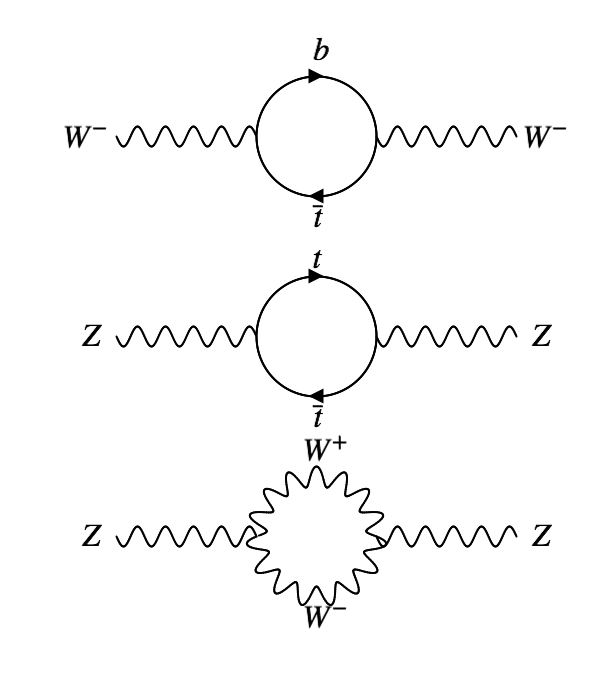
\includegraphics[width=0.75\textwidth]{images/web_feynman/image_84.png}
    \caption[Loops corrections for vector bosons]{Loops corrections for vector bosons.}
    \label{fig:ch16_vectorBosonLoops}
  \end{center}
\end{figure}

Measurements of $\rho$ yielded estimates of the top mass and now yields estimates of the Higgs mass.

\subsection{The coupling of the Higgs to the \texorpdfstring{$W^{\pm}$}{Wpm} and \texorpdfstring{$Z^0$}{Z0}}

Consider the Langrangian as:

\[
  \phi = \frac{1}{\sqrt{2}}
  \left(
  \begin{array}{c}
    0 \\
    \nu + h
  \end{array}
  \right)
\]

The $\partial_{\mu}$ term is then:

\begin{eqnarray*}
  & &
  \frac{1}{8}\left|
  \left(
  \begin{array}{cc}
    g_W W_{\mu}^3 + g' B_{\mu} & g_W\left(W_{\mu}^1 + iW_{\mu}^2\right) \\
    g_W \left(W_{\mu}^1 - iW_{\mu}^2\right) & -g_W W_{\mu}^3 + g'B_{\mu}
  \end{array}
  \right)
  \left(
  \begin{array}{c}
    0 \\
    \nu + h
  \end{array}
  \right)
  \right|^2
  \\
  & = & \frac{1}{8}\left(g_W^2\left(\nu + h\right)^2\left(W_{\mu}^1 - iW_{\mu}^2\right)\left(W_{\mu}^1 + W_{\mu}^2\right) - \left(\nu + h\right)^2\left(g'B_{\mu} - g_W W_{\mu}^3\right)\left(g'B^{\mu} - g_W W^{\mu}_3\right)\right)
\end{eqnarray*}

The weak-Higgs couping is:

\[
  \frac{1}{8}g_W^2\left(\left(\nu^2 + 2\nu h + h^2\right)\sqrt{2}W^+\sqrt{2}W^-\right)
\]

So there are trilinear ($WWH$) and quadrilinear ($WWHH$) couplings:

\begin{figure}[!htb]
  \begin{center}
    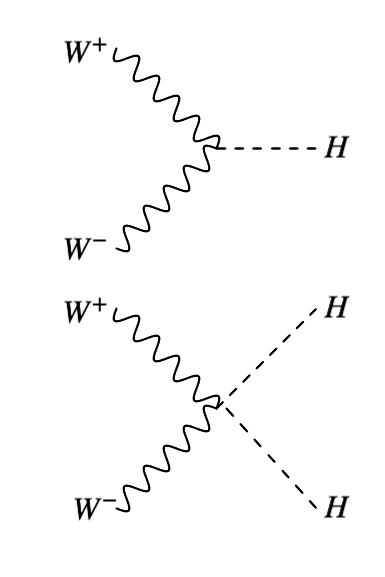
\includegraphics[width=0.5\textwidth]{images/web_feynman/image_85.png}
    \caption[Trilinear and quadrilinear Higgs-$W$ couplings]{Trilinear (top) and quadrilinear (bottom) Higgs-$W$ couplings.}
    \label{fig:ch16_WHiggs}
  \end{center}
\end{figure}

\begin{eqnarray*}
  coupling & = & \frac{1}{8}g_W^2 \times 2\nu h \sqrt{2}W^+\sqrt{2}W^- \\
  & = & g_WM_WhW^+W^-
\end{eqnarray*}

\begin{eqnarray*}
  coupling & = & \frac{1}{8}g_W^2 h^2 \\
  & = & \frac{1}{4}g_W^2 h^2 W^+W^-
\end{eqnarray*}

\subsection{Fermion masses}

In the Weinberg formulation the scalar field whose symmetry is spontaneously broken has hypercharge $Y = 1$ and allows a mechanism for giving masses to fermions.

The scalar field can be used to generate masses by connecting singlet and doublet states:

\begin{eqnarray*}
  L & = & -G_{\e} \left( \bar{\nu}_{\e} , \bar{\e}\right)_L\frac{1}{\sqrt{2}}
  \left(
  \begin{array}{c}
    0 \\
    \nu + h
  \end{array}
  \right)
  \e_R + \bar{\e}_R\left(0 , \nu + h \right)
  \left(
  \begin{array}{c}
    \nu_{\e} \\
    \e
  \end{array}
  \right)
  \\
  & = & -\frac{G_{\e}}{\sqrt{2}}\nu\left(\bar{\e}_R\e_L + \bar{\e}_L\e_R\right) - \frac{G_{\e}}{2}\left(\bar{\e}_L\e_R + \bar{\e}_R\e_L\right)h
\end{eqnarray*}

Now choose $G_{\e}$ such that:

\[
  \mathrm{m}_{\e} = \frac{G_{\e}\nu}{\sqrt{2}}
\]

and hence generate the electron mass:

\[
  L = -\mathrm{m}_{\e} \bar{\e} \e - \frac{\mathrm{m}_{\e}}{4} \bar{\e}\e h
\]

$G_{\e}$ is arbitrary so $\mathrm{m}_{\e}$ is not predicted.

The $d$ quark mass can be generated in the same way.  For the $u$ quark the symmetry is broken by choosing $\phi = \frac{1}{\sqrt{2}}\left(\begin{array}{c}\nu + h \\ 0 \end{array}\right)$ which has the opposite hypercharge ($Y = -1$) to previously.  Then a right-handed singlet $u$ quark can be connected to the left-handed doublet state $u$ quark.  Again this gives a Dirac-like mass term.

Starting with the weak eigenstates the mass generation of the quarks can be generalised.  The mass is generated by:

\[
  \bar{d}_L \bar{M}_d d'_R
\]

where $d$ represents the $d$ type quarks and $\bar{M}_d$ is a $3 \times 3$ matrix.  Also for $u$ type quarks::

\[
   \bar{u}'_L \bar{M}_u r'_R
\]

Consider the relationship between the weak and mass eigenstates:

\begin{eqnarray*}
  u_L & = & U^u_L u'_L \\
  u_R & = & U^u_R u'_R \\
  d_L & = & U^d_L d'_L \\
  d_R & = & U^d_R d'_R
\end{eqnarray*}

where the $U$s are $3 \times 3$ unitary matrices.

\[
  \textrm{So } \bar{u}_L' \bar{M}_uu_R' = \bar{u}_L \underbrace{U^u_L \bar{M}_u U^u_R{}^{\dagger}}_{\bar{M}}r_R
\]

where $\bar{M}$ is a diagonal matrix of quark masses.

Recall the nature of the charged current for quarks, first in terms of the weak eigenstates:

\[
  \left( \bar{u}' \quad \bar{c}' \quad \bar{t}' \right)
  \frac{1}{2}\gamma^{\mu}\left(1 - \gamma^5\right)
  \left(
  \begin{array}{c}
    d' \\
    s' \\
    b'
  \end{array}
  \right)
\]

In terms of the mass eigenstates:

\[
  \left( \bar{u} \quad \bar{c} \quad \bar{t} \right)
  U^u_L \frac{1}{2}\gamma^{\mu}\left(1 - \gamma^5\right) \left(U^d_L\right)^{\dagger}
  \left(
  \begin{array}{c}
    d \\
    s \\
    b
  \end{array}
  \right)
\]

In the weak interaction:

\[
  V_{CKM} = U^u_L\left(U^d_L\right)^{\dagger}
\]

The CKM matrix is related to the transformation which gives quarks their mass.

\section{A cosmological problem}

Recall that the Higgs well depth is given by $V_0 = -\frac{\lambda \nu^4}{4}$

Consider $\nu$.

\begin{eqnarray*}
  \textrm{Recall }\nu & = & \frac{2M_W}{g_W} \\
  g_W^2 & = & \frac{G_F \times 8M_W^2}{\sqrt{2}} \\
  \Rightarrow \nu & =& \frac{2}{\sqrt{\frac{8G_F}{\sqrt{2}}}} \\
  & = & 246 \gev \\
  \Rightarrow V_0 & = & -\frac{\lambda}{4}\nu^4 \\
  & \simeq & -\lambda \times 1.3 \times 10^{50}\units{\gev cm}^{-3}
\end{eqnarray*}

The visible desnity of the universe is $1$ photon per cubic metre $\sim 10^{-6} \gev cm^{-3}$, with dark matter and energy accounting for around $20$ times this amount.  Therefore the density in the Higgs field is $10^{55} \times \lambda$ larger than that in the universe (where $\lambda \sim \frac{1}{10}$ is taken to be a reasonable number.)

\section{Lagrangian of the Standard Model (Weinberg-Salam)}

\begin{eqnarray*}
  L & = & -\frac{1}{4}W_{\mu\nu}W^{\mu\nu} - \frac{1}{4}B_{\mu\nu}B^{\mu\nu} \\ \nopagebreak
    &   & \textrm{ $W$, $Z$, $\gamma$ kinetic energies and self-interactions} \\\nopagebreak
    & + & \bar{L}\gamma^{\mu}\left(i\partial_{\mu}-g\frac{\tau}{2}W_{\mu}-g'\frac{Y}{2}B_{\mu}\right)L + \bar{R}\gamma^{\mu}\left(\partial_{\mu} - g'\frac{Y}{2}B_{\mu}\right)R \\\nopagebreak
    &   & \textrm{ Lepton and quark kinetic energy and their interaction with $W$, $Z$, $\gamma$} \\\nopagebreak
    & + & \left|\left(i\partial_{\mu}-g\frac{\tau}{2}W_{\mu}-g'\frac{Y}{2}B_{\mu}\right)\phi\right|^2 - V(\phi) \\\nopagebreak
    &   & \textrm{ $W$, $Z$, $\gamma$, $H$ masses and couplings} \\\nopagebreak
    & - & \left(G_1 \bar{L}\phi R + G_2 \bar{L}\phi_C R' + \textrm{Hermitian conjugate}\right) \\\nopagebreak
    &   & \textrm{ Lepton and quark masses and couplings to Higgs}
\end{eqnarray*}

\section{Grand unification}

The electroweak $SU(2) \otimes U(1)$ theory is in impressive agreement with experiment, including many measurements from current colliders.  However the theoretical unification is not complete: the $SU(2)$ group has coupling strength $g$ and the $U(1)$ group has coupling strength $g'$, the relation of which is not predicted by theory, the ratio:

\[
  \frac{g'}{g} = \tan\theta_W
\]

is determined from experiment.  Only if there is a larger set of gauge transformations which embed $g$ and $g'$ can it be said that electromagnetism and the weak interaction are truly unified.

In attempting to unify the two forces in such a way, the strong force can also be considered and a Grand Unified Theory which encompasses all groups can be proposed:

\[
  \textrm{So }G \textrm{ or } SU(5) \supset SU(3) \otimes SU(2) \otimes U(1)
\]

where there is one coupling constant.  This implies that the couplings of each of the forices at some scale are equal.  Knowing the values at low energies and their variation with energy, this scale is $M_{GUT} \sim 10^{15}\gev$.

The simplest form of the $SU(5)$ group has been ruled out (the decays of $\e$ and $\pi$ are completely inconsistent between experiment and theory) but could still be valid as part of another scheme such as $SO(10)$.

In $SU(5)$, the $d$ quarks and the anti-lepton doublet are combined into a quintuplet:

\[
  \left(
  \begin{array}{c}
  d_R \\ d_B \\ d_G \\ \e^+ \\ \bar{\nu}_{\e}
  \end{array}
  \right)
\]

To allow local gauge transformations on this quintuplet fields have to be introduced combined with their corresponding $5 \times 5$ generators.

The $SU(5)$ group has $24$ independent generators, which are combined in $24$ fields:

\[
  \left(
  \begin{array}{ccc|cc}
    \star & \star & \star & \star & \star \\
    \star & SU(3) & \star &  (b)  & \star \\
    \star & \star & \star & \star & \star \\
    \hline
    \star &  (a)  & \star & SU(2) & \star \\
    \star & \star & \star & \star & \star \\
  \end{array}
  \right)
  \left(
  \begin{array}{c}
    d_R \\
    d_B \\
    d_G \\
    \hline
    \e^+ \\
    \nu_{\e}
  \end{array}
  \right)
\]

$(a)$ and $(b)$ can change leptons into quarks and vice-versa.  There are $12$ new gauge bosons: $X$ and $Y$ which allow for lepton-quark transition and have charges $Q_X = \pm\frac{4}{3}$ and $Q_Y = \pm \frac{1}{3}$.

The charge generator $Q$ must be a linear combination of the diagonal genertors in $SU(5)$:

\begin{eqnarray*}
  Q & = & T_3 + \frac{Y}{2} \\
    & = & T_3 + cT_0
\end{eqnarray*}

where $T_3$ (isospin) and $T_0$ are the diagonal generators of $SU(5)$ belonging to the $SU(2)$ and $U(1)$ subgroups.  The coefficient $c$ relates the operators $Y$ and $T_0$ and has the value $\sqrt{\frac{5}{3}}$.

The diagonal generator is:

\[
  \sqrt{\frac{3}{5}}
  \left(
  \begin{array}{ccccc}
    -\frac{2}{3} & 0 & 0 & 0 & 0 \\
    0 & -\frac{2}{3} & 0 & 0 & 0 \\
    0 & 0 & -\frac{2}{3} & 0 & 0 \\
    0 & 0 & 0 & 1 & 0 \\
    0 & 0 & 0 & 0 & 1
  \end{array}
  \right)
\]

\begin{eqnarray*}
  Tr[\cdots][\cdots] & = & 2\delta_{ij} \\
  \textrm{ie } N^2\left(\frac{4}{9} + \frac{4}{9} + \frac{4}{9} + 1 + 1\right) & = & 2 \\
  \Rightarrow N & = & \sqrt{\frac{3}{5}}
\end{eqnarray*}

The unified coupling constant is $g_5$, where:

\begin{eqnarray*}
  g_W & = & g_5 \\
  g_s & = & g_5 \\
  g'  & = & \sqrt{\frac{3}{5}} g_5 \\
      & = & \sqrt{\frac{3}{5}} g_W \\
  \textrm{But } g'\cos\theta_W & = & g_W\sin\theta_W \\
  \Rightarrow \tan\theta_W & = & \sqrt{\frac{3}{5}}
\end{eqnarray*}

This is at the unification energy.  Evolution back to low energies shows that the theory does not quite match the data.

Similarly assuming that the interaction $g_1(Y)$, $g_2 = g_W$ and $g_3 = g_5$ are unified to $g_5$, then their evolution down to current energies can be predicted.

\begin{eqnarray*}
  \frac{1}{\alpha_3(Q^2)} & = & \frac{1}{\alpha_3(M^2)} + \frac{1}{4\pi}\left(11 - \frac{2}{3}n_g\right) \ln\left(\frac{Q^2}{M^2}\right) \\
  \frac{1}{\alpha_2(Q^2)} & = & \frac{1}{\alpha_2(M^2)} + \frac{1}{4\pi}\left(\frac{22}{3} - \frac{4}{3}n_g\right) \ln\left(\frac{Q^2}{M^2}\right) \\
  \frac{1}{\alpha_1(Q^2)} & = & \frac{1}{\alpha_1(M^2)} + \frac{1}{4\pi}\left( - \frac{4}{3}n_g\right) \ln\left(\frac{Q^2}{M^2}\right) \\
\end{eqnarray*}

\begin{figure}[!htb]
  \begin{center}
    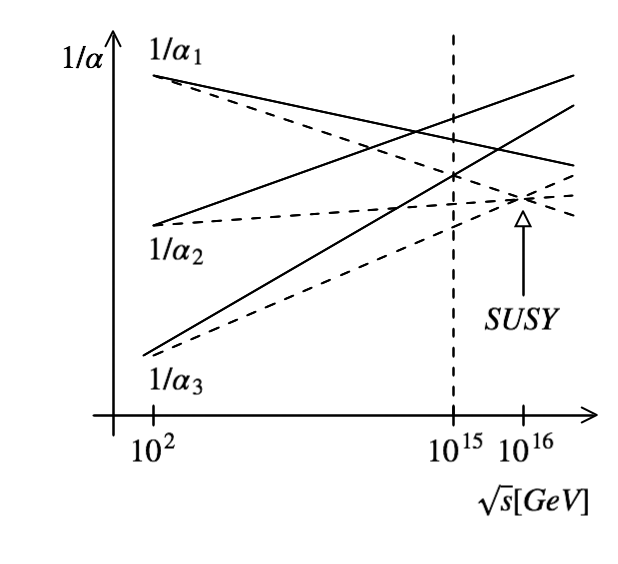
\includegraphics[width=\textwidth]{images/web_feynman/image_86.png}
    \caption[SUSY and unification at high energy]{Evolution of the couplings under a SUSY scenario and unification at high energy.}
    \label{fig:ch16_SUSYUnification}
  \end{center}
\end{figure}

In fact the coupling constants do not meet at the GUT scale. Also, had they met at $10^{15}\gev$ this would imply that protons would decay with lifetimes of $\sim 10^{31}$ years, which is ruled out by experiment.

This could be evidence for super-symmetry ie each boson has a fermion partner and vice versa.  Such particles would slow down evolution of the coupling constants.
